\section{Photogrammetry and Unmanned Aerial Systems}
Generically, an Autonomous Air System (UAS) is composed of a ground control station (GCS), a communications system and an aerial element (UAV- Unmanned aerial vehicle). The operation of the system is based on the fact that an operator at the ground control station directs a Datalink to operate the UAV based on the information relayed by the UAV through its sensors. Depending on performance characteristics of the UAV such as service ceiling, speed, scope, coverage, transmission capacity of the data link, autonomy, and decision-making capacity of the UAV, the system operation varies.\cite{Duran}
\begin{figure}[H]
\centering
\includegraphics[width=15cm,height=15cm,keepaspectratio]{imagenes/UAS_Components.png}
\caption{UAS Block diagram.}
\label{fig:block diagram}
\end{figure}

\subsection{UAS components}
As previously described, there are three main components to a UAS: Ground Control Station (GCS), Data Link (communications system) and aerial element. This section presents a description of each component.
\subsubsection{Ground segment} 
The ground control station is where the operator interacts with a UAS. It comprises several parts, usually providing feedback about UAV activity, allowing command and control of the aerial element and providing for a method to override control for the system.
The GCS can be divided into the following components:
\begin{itemize}
    \item \textbf{Ground Computer:} is the computer or system where the ground station software is executed, also where the downlink of the Datalink is received.
    \item \textbf{Ground Software:}  ground software on the GCS provides the human interface for configuration, monitoring, and control of the UAS. The ground software should provide:
    \begin{itemize}
        \item Compilation tools to produce the airborne software from the configurations and source code.
        \item GUI to control and interact with the UAV(s) during flight as well as mission planning and simulation.
        \item Basic simulator to ease the development of flight plans and verify airborne code behavior.
        \item Data logging system with a plot-based viewer for real-time and post-flight analysis.
        \item Number of utilities for communicating with the UAV and other agents.
        \item Number of tools for calibration.
        \item Control panel GUI for configuration and program management.
    \end{itemize}
    \item \textbf{Groundside Datalink:} offers possibilities to supervise the UAV flight from the ground. By default, it uses a bidirectional wireless modem which supports both telemetry (downlink) and tele control (uplink). Thanks to this data link, flight parameters are available in real time. It is also possible to fully control the navigation and tuning of one, or several air elements from the ground station. The ground side of the link usually consists of a matching radio modem, like an XBee, connected to the ground control station computer over USB or serial port.
    \item \textbf{Groundside Safelink:} The ground side of the safety link usually consists of a radio control transmitter (and safety pilot). It is used to provide manual control of the UAV.
\end{itemize}
\subsubsection{Data link}
The UAS data link is a system for monitoring control and information transmission. Generally, it consists of the link protocol, the transport channel and the message protocol. It is designed to achieve real-time information exchange between the sensors, GCS and the UAV as well as to handle the information from flying scene situation, command control, and mission control.\cite{6305636} The data link can be divided into two: \textit{Downlink} and \textit{Uplink}:

\begin{itemize}
    \item \textbf{Donwlink:}  is used to transmit the information from the UAV to the GCS, including status, sensor, and graphic image data. In general, the UAV is controlled mainly by the onboard autopilot, with the GCS being used to monitor the flight status and handling of an emergency. \cite{6305636}
    \item \textbf{Uplink:} is used to transmit the control information from the GCS to the UAV, such as flight parameters, way-point information and command instructions. \cite{6305636}
\end{itemize}

The UAS transmission channel consists of two parts: the data terminal equipment (DTE) and the wireless channel. DTE, composed by a modem, network controllers and cryptographic equipment, is the fundamental and essential unit of the data link. The operating frequencies of data link are usually in HF, VHF, UHF, L, S, C, and K band, and the choice of frequency depends on its entrusted mission and technology system.\cite{6305636}

The radio modem is the most common DTE in small civilian UAS. It embodies the function of radio transmission, digital modulation and error correction; provides a serial transmission with the rate between 9600 bps and 19200 bps, as well as supporting half-duplex or full-duplex communication.\cite{6305636}

There is a third data link in a UAS system called \textit{Safe Link}. A traditional radio control transmitter and receiver(RC) pair are used to provide a manual control option to the UAV. The airborne hardware and software support the connection to a standard radio-control receiver. The autopilot reads the output from the R/C receiver on board the UAV and decides what the desire control mode should be. While in manual mode, a safety pilot on the ground may use the R/C transmitter to control the UAV. The fly-by-wire mode provides a reliable method of providing override control even though the autopilot always remains inline between R/C receiver and actuators.\cite{Hattenberger2014UsingTP}

\subsubsection{Airbone segment}
The airborne segment comprises the UAV, its hardware including payload and all the embedded software to control the flight (from stabilization to decision making). The key components are:
\begin{itemize}
    \item Autopilot board.
    \item Altitude sensor.
    \item Inertial Measurement Unit (IMU).
    \item GPS Receiver.
    \item Datalink Radio Modem.
    \item RC receiver.
    \item Servos.
    \item Propulsion system.
    \item Batteries.
    \item Payload.
\end{itemize}
For this project, the most relevant components are the autopilot, payload, and propulsion system. Comprises as follows:
\begin{figure}[H]
\centering
\includegraphics[width=10cm,height=10cm,keepaspectratio]{imagenes/opterra.jpg}
\caption{Opterra fixed-wing UAV.}
\label{fig:Optera}
\end{figure}
\textbf{ Autopilot} or controller board, is the system responsible for carrying out all the tasks on the UAV for the control, it can be said that it is the brain of the UAS. Its main functions are: Controlling the propulsion system and the stability of the UAV, managing communication with the control station and executing the instructions of the pilot. The CPU works with other modules of the flight management system, collecting information from a series of MEMS sensors (Micro-Electromechanical Systems) and receives satellite navigation status, in order to estimate the position and orientation of the UAV system. Also establishes a communication link with the control station through a module of radio frequency.\cite{Edgar}

The autopilot, in conjunction with the other blocks, must have the ability to:
\begin{itemize}
    \item Measure and estimate the orientation and spatial location of the system.
    \item Generate control signals to the actuators during the flight.
    \item Control and monitoring of the flight route.
    \item Monitoring and sending the conditions of the UAV through the communication link.
    \item Control of pilot instruction.
    \item Operate sensors.
\end{itemize}

The project utilizes the Apogee autopilot. Apogee is the latest in French Engineering and Design from E.N.A.C.  This controller uses the latest STM32F4 processor to create a complete autopilot controller board. \cite{apogee}
\begin{figure}[H]
\centering
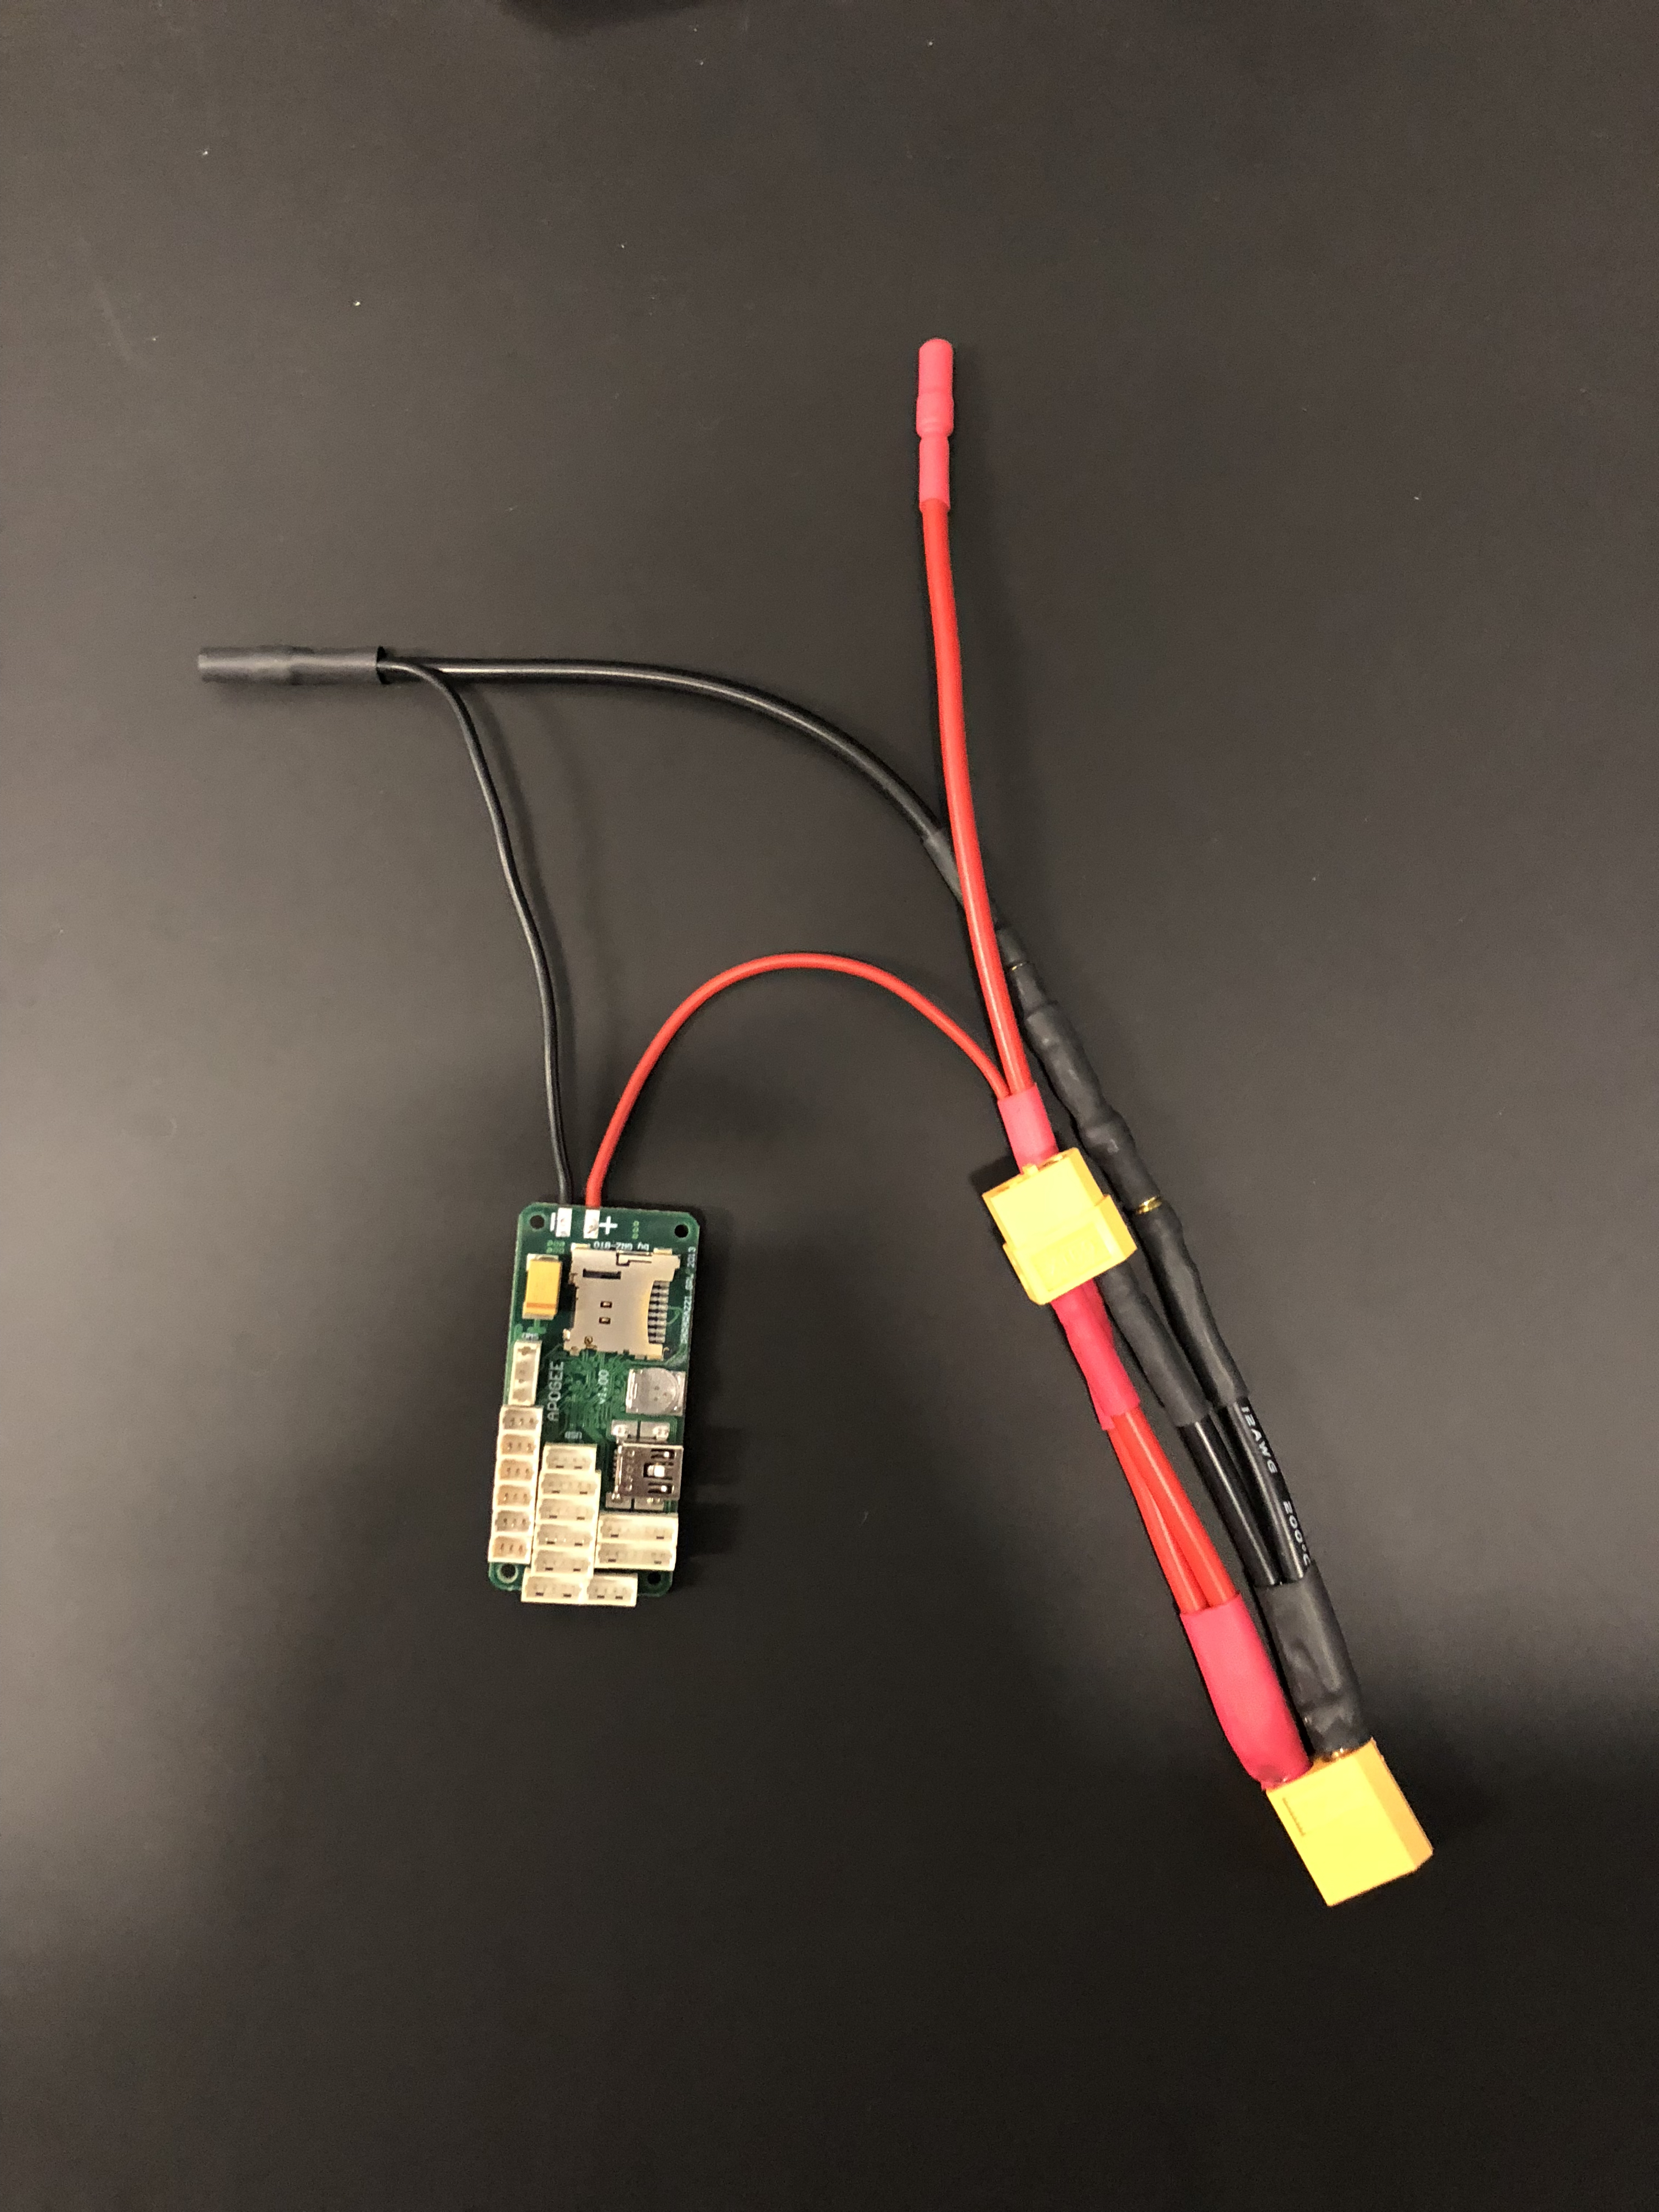
\includegraphics[width=10cm,height=10cm,keepaspectratio]{imagenes/apogee.jpg}
\caption{Apogee autopilot.}
\label{fig:apogee}
\end{figure}
As mentioned before, one of the main tasks performed by the autopilot is the controlling and monitoring the flight route. The guidance, navigation, and control of the UAV are implemented utilizing the \textit{Guiding Vector Field (GVF)} algorithm. 

The vector field algorithms are widely used in many applications in robotics such as path-planning, obstacle avoidance, and extremum seeking. The main idea is to design a potential vector field, whose integral lines converge to the desired path. In particular, the general description of the vector field for the path following.\cite{GVF}

Guidance vector field approach, which originates in a potential field method, provides an efficient and convenient way for the path following problem. It assigns a desired path angle for each point in the space. This desired path angle is usually a function of the coordinates of the corresponding point. Moreover, a series of these desired path angles determine the desired trajectory, and by tracking this trajectory, the path following objective can be finally achieved.\cite{7170894}

For fixed-wings, the output of the algorithm can be directly expressed in terms of the bank angle of the UAV to achieve coordinated turns. Furthermore, the algorithm can be tuned offline such that the physical constraints of the UAV, e.g., the maximum bank angle, does not violate in a neighborhood of the desired trajectory.\cite{7942030}


\textbf{Payload} virtually all kinds of payloads can be attached to the UAV, the only restrictions being the weight and size of payloads. Most UAV's are equipped with cameras. For this project, the payload is a camera pointed downwards, placed on the "belly" of the UAV. 

The UAV can be categorized by different criteria: 
\begin{itemize}
    \item \textbf{Propultion type.}
    \item  \textbf{Maximum take-off weight.}
\end{itemize}
\textbf{Propulsion type} can be divided into two main categories:
\begin{itemize}
\item Fixed-wing UAS: Fixed-wing UAV are characterized for having a highly efficient aerodynamic structure, that allows it to reach higher speeds than multirotor platforms, due to lower power consumption. The landing and take-off procedure present a difficulty in these types of UAV due to the necessity of a runway.
\item Rotatory wing: They are composed of 2 or more rotors. Its main characteristics are the ability to perform vertical take-off and landings, in addition to having great maneuverability and flight precision. Its main disadvantage is having a more complex electronics structure which sacrifices flight autonomy.\cite{Luis_Fernadno}
\end{itemize}

\textbf{Maximum take-off Weight}: The first classification to be established for UAV is based on the vehicle size. According to these criteria, they are a high number of platforms that can be categorized as mini, micro, small or large dimension. Maximum Take-Off Weight (MTOW) is the parameter used to classify the UAV. MTOW is the sum of UAV weight, maximum payload, and power unit.\cite{ICAO}

\subsection{Photogrammetry}
There is no formal definition for the term photogrammetry but  can be described as the science that focuses on obtaining  reliable information from objects or surfaces without having physical contact a the same time.\cite{Fotogrametria_digital}

Photogrammetry allows one to reconstruct the position, orientation, shape, and size of the object; these pictures may originate as photochemical images (conventional photography) or as photoelectrical images (digital photography). Laser scanner images, a third group, have arrived in recent years; laser scanner images have distances information associated with every picture element. The result of a photogrammetric analysis may be:\cite{Kraus}
\begin{itemize}
    \item Numbers: coordinates of separate points in a three-dimensional system (digital point determination).
    \item Drawings (analog):  maps and plan with planimetric detail and contour lines together with other graphical representation of objects.
    \item Geometric models (digital): which are fed into the information system.
    \item Images (analog and/or digital): above all, rectified photographs (orthophotos) and,and its derivatives, photmaps  as well as photomontages and so called three-dimensional photo models, which are textured CAD models with textures extracted from photographs.
\end{itemize}
That branch of photogrammetry which uses conventional photographs employs optical and mechanical processing instruments is called analog photogrammetry. The one based on conventional photographs which resolves the complete process of analysis employing computers is called analytical photogrammetry. The third stage of development is digital photogrammetry. In that case. Starting from such digital photographs, the whole process of evaluation is employing computers. Photogrammetry has some connection with machine vision, or computer vision, in which pattern recognition is one aspect.\cite{Kraus} 

In many cases, the interpretation of the content of the images goes hand in hand with the geometrical reconstruction of the photographed object. The outcome of such photointerpretation is the classification of objects within the images according to different characteristics.\cite{Kraus}

Photogrammetry allows the reconstruction of an object and the analysis of its characteristics without physical contact with it. Acquisition of information about the surface of the Earth in this way is known nowadays as remote sensing. Remote sensing embraces all methods of acquiring information about the Earth's surface employing measurement and interpretation of electromagnetic radiation either reflected from or emitted by it. While remote sensing includes that part of photogrammetry which concerns itself one speaks of photogrammetry and not of remote sensing. \cite{Kraus}

\begin{figure}[H]
\centering
\includegraphics[width=10cm,height=10cm,keepaspectratio]{imagenes/Photogram.png}
\caption{Conceptual outline about the procedure to perform an aerial photogrammetric survey\cite{pulicacion}.}
\label{fig:photogrametry}
\end{figure}